\documentclass[11pt]{article}
\usepackage[utf8]{inputenc}
\usepackage[margin=1in]{geometry}
\usepackage{listings}
\usepackage{xcolor}
\usepackage{graphicx}
\usepackage{hyperref}
\hypersetup{
    colorlinks=true,
    linkcolor=blue,
    filecolor=magenta,      
    urlcolor=blue,
}

% Define colors for code blocks
\definecolor{codegreen}{rgb}{0,0.6,0}
\definecolor{codegray}{rgb}{0.5,0.5,0.5}
\definecolor{codepurple}{rgb}{0.58,0,0.82}
\definecolor{backcolour}{rgb}{0.95,0.95,0.92}

\lstdefinestyle{mystyle}{
    backgroundcolor=\color{backcolour},   
    commentstyle=\color{codegreen},
    keywordstyle=\color{magenta},
    numberstyle=\tiny\color{codegray},
    stringstyle=\color{codepurple},
    basicstyle=\ttfamily\small,
    breaklines=true,
    captionpos=b,                    
    keepspaces=true,                 
    numbers=left,                    
    showspaces=false,                
    showstringspaces=false,
    showtabs=false,                  
    tabsize=2
}

\lstset{style=mystyle}

\title{Quick Start Guide: Accessing HDF5 Data}
\author{Pierre Bouvet}

\begin{document}

\maketitle

\section*{Introduction}

This guide explains how to open and retrieve data from any HDF5 file using Python and MATLAB, particularly the HDF5 files following the guidelines presented in the \href{https://github.com/bio-brillouin/HDF5_BLS}{HDF5\_BLS} project.

In short a HDF5 file is a container for data that can be organized in a hierarchical structure. It is a great option to organize in a single file a large amount of arrays and attributes. 

\section{Step 1 - Simple visualization using myHDF5}

Before any further step, we recommend using the \href{https://myhdf5.hdfgroup.org/}{myHDF5 viewer} to preview the file, its components, and its hierarchy.
\begin{enumerate}
    \item Go to \href{https://myhdf5.hdfgroup.org/}{myHDF5 viewer}
    \item Drag and drop your file
    \item Navigate your file through the web application
\end{enumerate} 

You should see something like:

\begin{figure}[h]
    \centering
    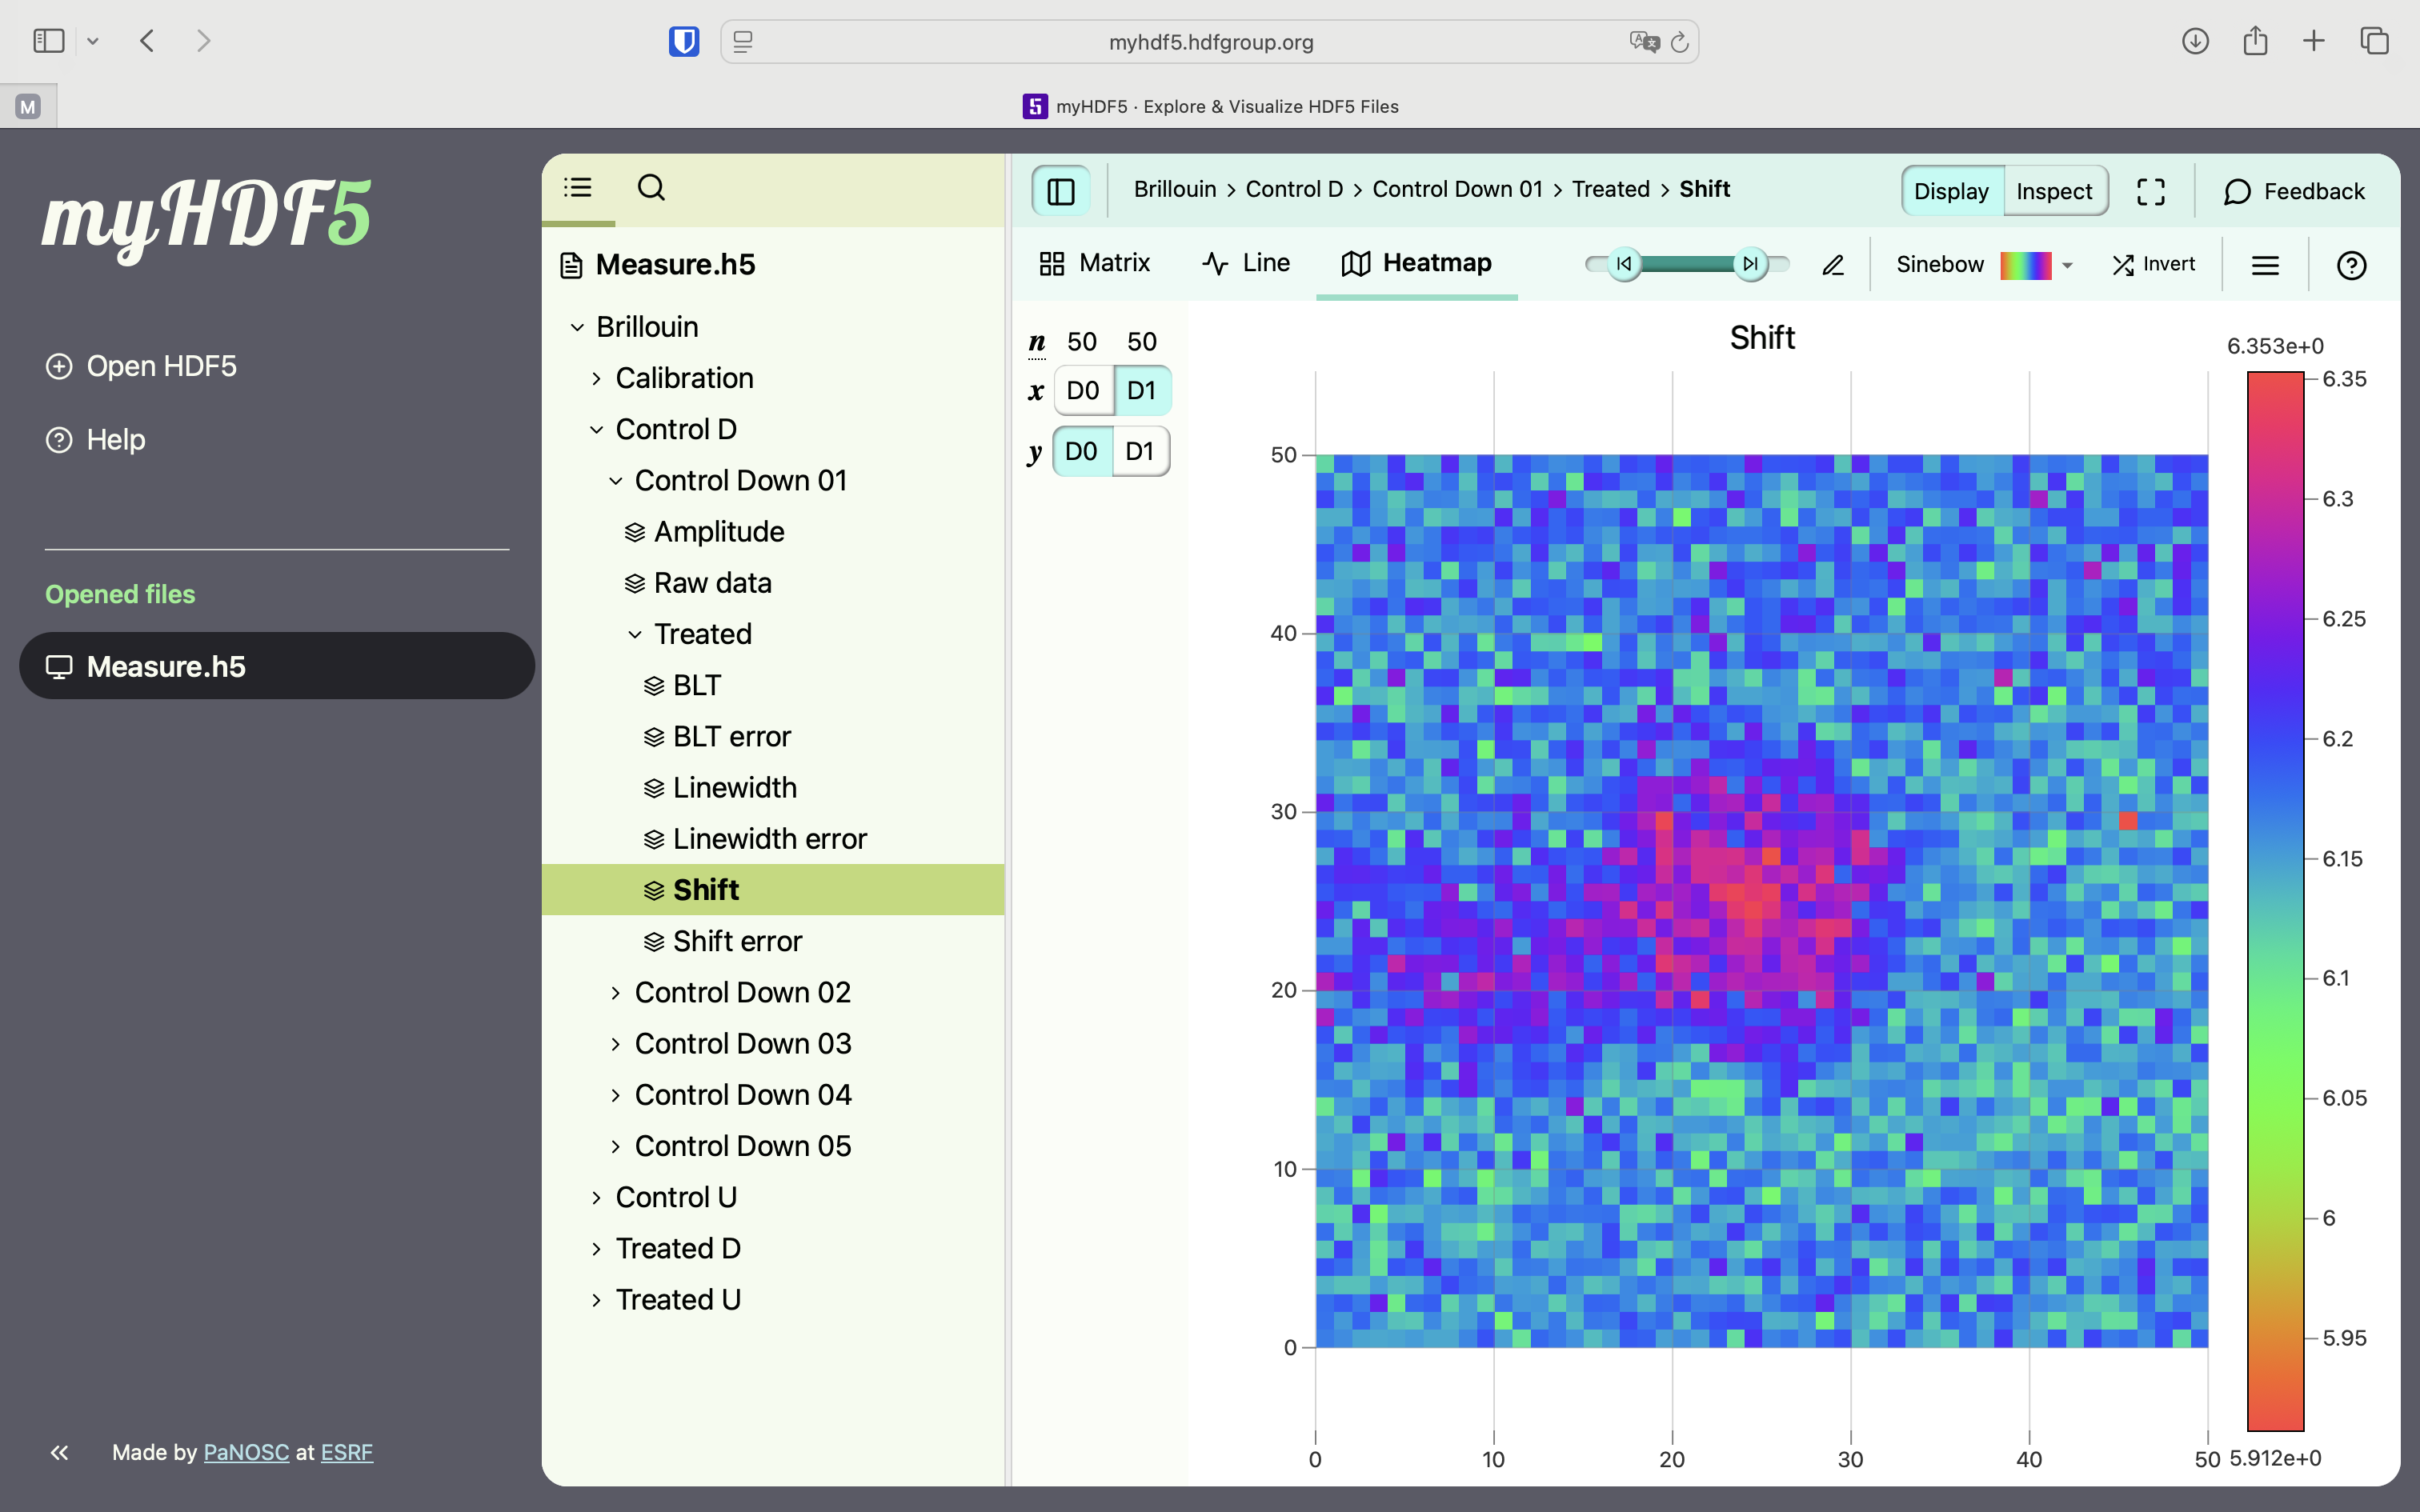
\includegraphics[width=0.7\textwidth]{img/myHDF5_Architecture.png}
    \caption{Example of HDF5 file structure in myHDF5 viewer}
    \label{fig:hdf5_structure}
\end{figure}

\subsection{Step 2 - Locating the Dataset Path}
HDF5 uses a Unix-style path system. To get the exact path for your code:
\begin{enumerate}
    \item Select the dataset in the Tree View.
    \item Navigate to the "Inspect" tab (top right)
    \item Get the "Path" field (e.g., \texttt{/group\_name/subgroup/dataset\_name}).
\end{enumerate}

For example here:
\begin{figure}[h]
    \centering
    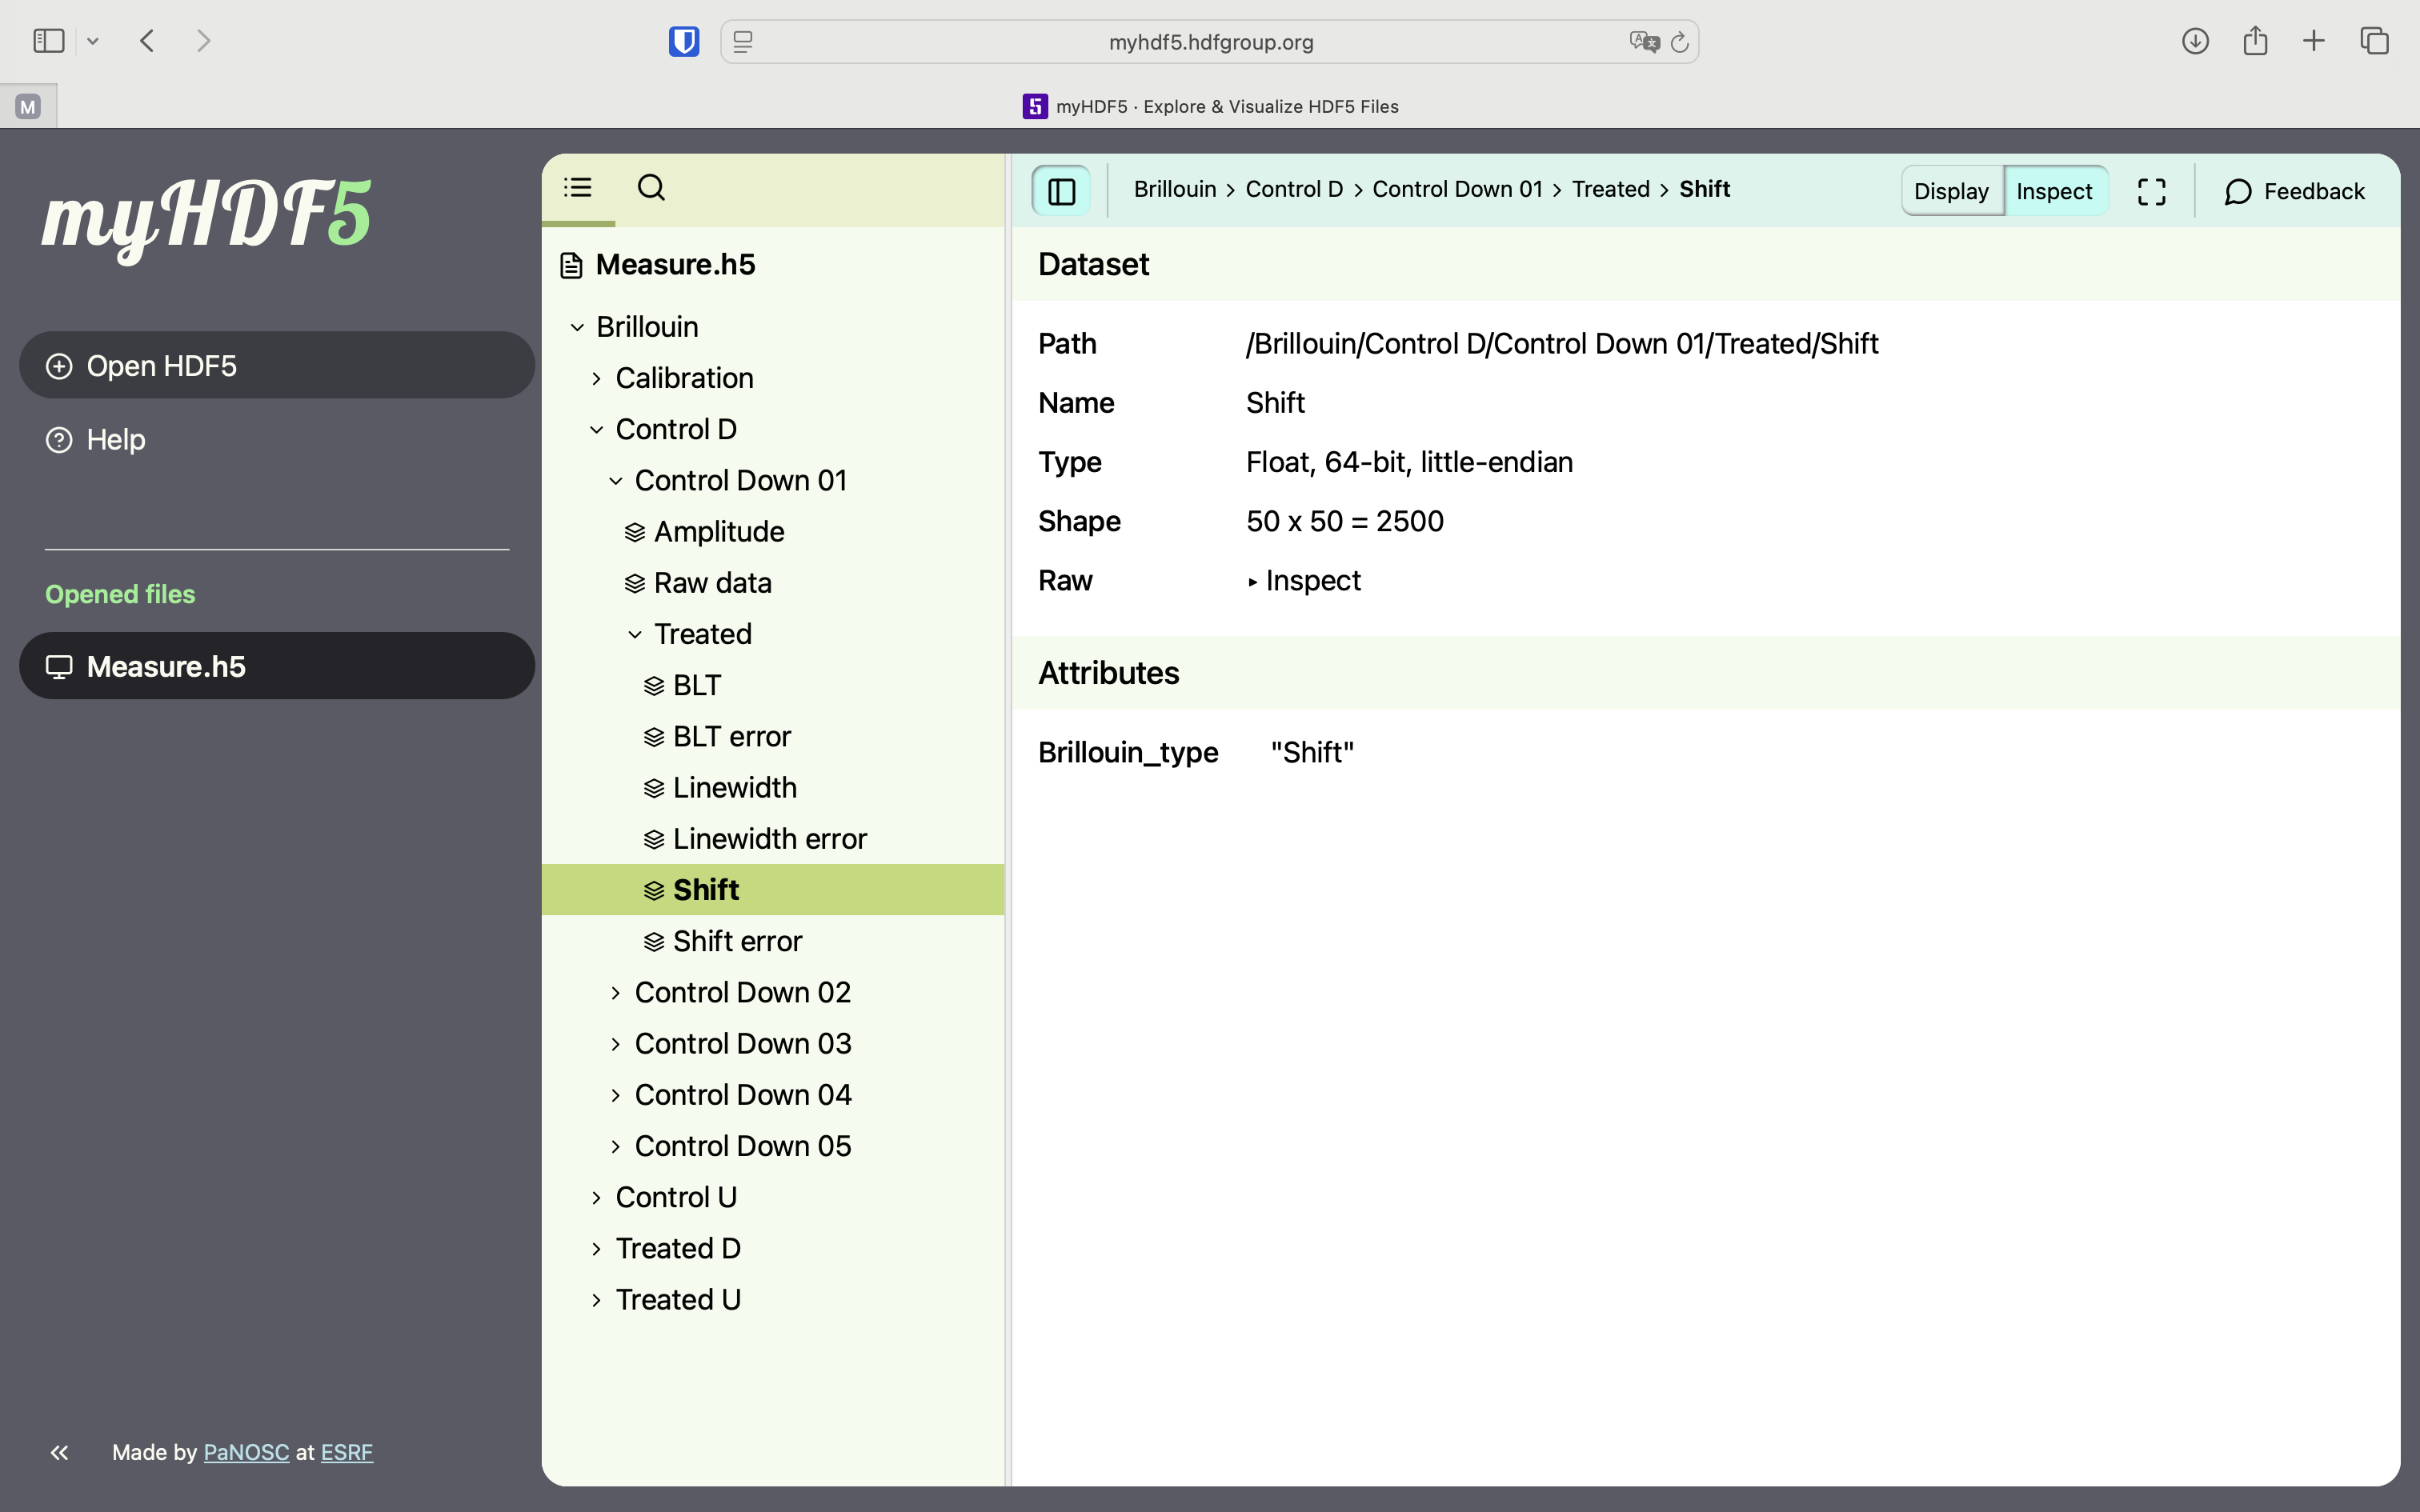
\includegraphics[width=0.7\textwidth]{img/myHDF5_Path.png}
    \caption{Example of HDF5 file structure in myHDF5 viewer}
    \label{fig:hdf5_structure}
\end{figure}
the path is: "/Brillouin/Control D/Control Down 01/Treated/Shift"

\newpage

\section{Step 2 - Extracting Data via Code}
Once you have the path from myHDF5, use the following snippets to pull the data into your workspace.

\subsection{Python (using h5py)}
Python requires the \texttt{h5py} library - you can install it using 'pip' writing the following line in the terminal: \texttt{pip install h5py}. 

Once h5py is installed, you can access your dataset as follows:

\begin{lstlisting}[language=Python, caption=Python extraction]
import h5py
import numpy as np

filename = "your_file.h5"
dataset_path = "/path/to/dataset" # Obtained from myHDF5

with h5py.File(filename, "r") as f:
    # Access the dataset and convert to a NumPy array
    data = f[dataset_path][()] 
\end{lstlisting}

\subsection{MATLAB}
MATLAB has built-in support via the \texttt{h5read} function, so no extra library have to be installed:

\begin{lstlisting}[language=Matlab, caption=MATLAB extraction]
filename = 'your_file.h5';
dataset_path = '/path/to/dataset'; % Obtained from myHDF5

% Read the data directly into a variable
data = h5read(filename, dataset_path);
\end{lstlisting}

\end{document}